% Options for packages loaded elsewhere
\PassOptionsToPackage{unicode}{hyperref}
\PassOptionsToPackage{hyphens}{url}
\PassOptionsToPackage{dvipsnames,svgnames,x11names}{xcolor}
%
\documentclass[
  letterpaper,
  DIV=11,
  numbers=noendperiod]{scrreprt}

\usepackage{amsmath,amssymb}
\usepackage{iftex}
\ifPDFTeX
  \usepackage[T1]{fontenc}
  \usepackage[utf8]{inputenc}
  \usepackage{textcomp} % provide euro and other symbols
\else % if luatex or xetex
  \usepackage{unicode-math}
  \defaultfontfeatures{Scale=MatchLowercase}
  \defaultfontfeatures[\rmfamily]{Ligatures=TeX,Scale=1}
\fi
\usepackage{lmodern}
\ifPDFTeX\else  
    % xetex/luatex font selection
\fi
% Use upquote if available, for straight quotes in verbatim environments
\IfFileExists{upquote.sty}{\usepackage{upquote}}{}
\IfFileExists{microtype.sty}{% use microtype if available
  \usepackage[]{microtype}
  \UseMicrotypeSet[protrusion]{basicmath} % disable protrusion for tt fonts
}{}
\makeatletter
\@ifundefined{KOMAClassName}{% if non-KOMA class
  \IfFileExists{parskip.sty}{%
    \usepackage{parskip}
  }{% else
    \setlength{\parindent}{0pt}
    \setlength{\parskip}{6pt plus 2pt minus 1pt}}
}{% if KOMA class
  \KOMAoptions{parskip=half}}
\makeatother
\usepackage{xcolor}
\setlength{\emergencystretch}{3em} % prevent overfull lines
\setcounter{secnumdepth}{5}
% Make \paragraph and \subparagraph free-standing
\makeatletter
\ifx\paragraph\undefined\else
  \let\oldparagraph\paragraph
  \renewcommand{\paragraph}{
    \@ifstar
      \xxxParagraphStar
      \xxxParagraphNoStar
  }
  \newcommand{\xxxParagraphStar}[1]{\oldparagraph*{#1}\mbox{}}
  \newcommand{\xxxParagraphNoStar}[1]{\oldparagraph{#1}\mbox{}}
\fi
\ifx\subparagraph\undefined\else
  \let\oldsubparagraph\subparagraph
  \renewcommand{\subparagraph}{
    \@ifstar
      \xxxSubParagraphStar
      \xxxSubParagraphNoStar
  }
  \newcommand{\xxxSubParagraphStar}[1]{\oldsubparagraph*{#1}\mbox{}}
  \newcommand{\xxxSubParagraphNoStar}[1]{\oldsubparagraph{#1}\mbox{}}
\fi
\makeatother


\providecommand{\tightlist}{%
  \setlength{\itemsep}{0pt}\setlength{\parskip}{0pt}}\usepackage{longtable,booktabs,array}
\usepackage{calc} % for calculating minipage widths
% Correct order of tables after \paragraph or \subparagraph
\usepackage{etoolbox}
\makeatletter
\patchcmd\longtable{\par}{\if@noskipsec\mbox{}\fi\par}{}{}
\makeatother
% Allow footnotes in longtable head/foot
\IfFileExists{footnotehyper.sty}{\usepackage{footnotehyper}}{\usepackage{footnote}}
\makesavenoteenv{longtable}
\usepackage{graphicx}
\makeatletter
\def\maxwidth{\ifdim\Gin@nat@width>\linewidth\linewidth\else\Gin@nat@width\fi}
\def\maxheight{\ifdim\Gin@nat@height>\textheight\textheight\else\Gin@nat@height\fi}
\makeatother
% Scale images if necessary, so that they will not overflow the page
% margins by default, and it is still possible to overwrite the defaults
% using explicit options in \includegraphics[width, height, ...]{}
\setkeys{Gin}{width=\maxwidth,height=\maxheight,keepaspectratio}
% Set default figure placement to htbp
\makeatletter
\def\fps@figure{htbp}
\makeatother
% definitions for citeproc citations
\NewDocumentCommand\citeproctext{}{}
\NewDocumentCommand\citeproc{mm}{%
  \begingroup\def\citeproctext{#2}\cite{#1}\endgroup}
\makeatletter
 % allow citations to break across lines
 \let\@cite@ofmt\@firstofone
 % avoid brackets around text for \cite:
 \def\@biblabel#1{}
 \def\@cite#1#2{{#1\if@tempswa , #2\fi}}
\makeatother
\newlength{\cslhangindent}
\setlength{\cslhangindent}{1.5em}
\newlength{\csllabelwidth}
\setlength{\csllabelwidth}{3em}
\newenvironment{CSLReferences}[2] % #1 hanging-indent, #2 entry-spacing
 {\begin{list}{}{%
  \setlength{\itemindent}{0pt}
  \setlength{\leftmargin}{0pt}
  \setlength{\parsep}{0pt}
  % turn on hanging indent if param 1 is 1
  \ifodd #1
   \setlength{\leftmargin}{\cslhangindent}
   \setlength{\itemindent}{-1\cslhangindent}
  \fi
  % set entry spacing
  \setlength{\itemsep}{#2\baselineskip}}}
 {\end{list}}
\usepackage{calc}
\newcommand{\CSLBlock}[1]{\hfill\break\parbox[t]{\linewidth}{\strut\ignorespaces#1\strut}}
\newcommand{\CSLLeftMargin}[1]{\parbox[t]{\csllabelwidth}{\strut#1\strut}}
\newcommand{\CSLRightInline}[1]{\parbox[t]{\linewidth - \csllabelwidth}{\strut#1\strut}}
\newcommand{\CSLIndent}[1]{\hspace{\cslhangindent}#1}

\KOMAoption{captions}{tableheading}
\makeatletter
\@ifpackageloaded{bookmark}{}{\usepackage{bookmark}}
\makeatother
\makeatletter
\@ifpackageloaded{caption}{}{\usepackage{caption}}
\AtBeginDocument{%
\ifdefined\contentsname
  \renewcommand*\contentsname{Table of contents}
\else
  \newcommand\contentsname{Table of contents}
\fi
\ifdefined\listfigurename
  \renewcommand*\listfigurename{List of Figures}
\else
  \newcommand\listfigurename{List of Figures}
\fi
\ifdefined\listtablename
  \renewcommand*\listtablename{List of Tables}
\else
  \newcommand\listtablename{List of Tables}
\fi
\ifdefined\figurename
  \renewcommand*\figurename{Figure}
\else
  \newcommand\figurename{Figure}
\fi
\ifdefined\tablename
  \renewcommand*\tablename{Table}
\else
  \newcommand\tablename{Table}
\fi
}
\@ifpackageloaded{float}{}{\usepackage{float}}
\floatstyle{ruled}
\@ifundefined{c@chapter}{\newfloat{codelisting}{h}{lop}}{\newfloat{codelisting}{h}{lop}[chapter]}
\floatname{codelisting}{Listing}
\newcommand*\listoflistings{\listof{codelisting}{List of Listings}}
\makeatother
\makeatletter
\makeatother
\makeatletter
\@ifpackageloaded{caption}{}{\usepackage{caption}}
\@ifpackageloaded{subcaption}{}{\usepackage{subcaption}}
\makeatother

\ifLuaTeX
  \usepackage{selnolig}  % disable illegal ligatures
\fi
\usepackage{bookmark}

\IfFileExists{xurl.sty}{\usepackage{xurl}}{} % add URL line breaks if available
\urlstyle{same} % disable monospaced font for URLs
\hypersetup{
  pdftitle={Desarrollo Web FontEnd},
  pdfauthor={T.S. Christopher Jara},
  colorlinks=true,
  linkcolor={blue},
  filecolor={Maroon},
  citecolor={Blue},
  urlcolor={Blue},
  pdfcreator={LaTeX via pandoc}}


\title{Desarrollo Web FontEnd}
\author{T.S. Christopher Jara}
\date{2024-09-25}

\begin{document}
\maketitle

\renewcommand*\contentsname{Table of contents}
{
\hypersetup{linkcolor=}
\setcounter{tocdepth}{2}
\tableofcontents
}

\bookmarksetup{startatroot}

\chapter*{Bienvenida}\label{bienvenida}
\addcontentsline{toc}{chapter}{Bienvenida}

\markboth{Bienvenida}{Bienvenida}

¡Bienvenido al Curso de Desarrollo Web, diseñado para los estudiantes de
tercero de bachillerato de la U.E.P. ``Carlos Crespi II, cursantes de la
materia de Desarrollo Web, especialidad Informática.

En este curso, exploraremos todo, desde los fundamentos, revisando las
herramientas de última tecnología, hasta las aplicaciones prácticas.

\section*{\texorpdfstring{\textbf{¿De qué trata este
curso?}}{¿De qué trata este curso?}}\label{de-quuxe9-trata-este-curso}
\addcontentsline{toc}{section}{\textbf{¿De qué trata este curso?}}

\markright{\textbf{¿De qué trata este curso?}}

Durante este periodo lectivo, cursaremos fundamentos teóricos básicos de
la programación hasta la construcción de sitios web completos utilizando
los lenguajes de programación HTML, CSS y JavaScript.

A través de una combinación de teoría y ejercicios prácticos, nos
sumergiremos en los conceptos esenciales del desarrollo web y
avanzaremos hacia la creación de proyectos del mundo real, con clientes
reales, mismos que aportaran con su retroalimentación, con lo que cada
proyecto se convertirá en una experiencia única.

Juntos recorreremos desde la configuración del entorno de desarrollo
hasta la construcción de un sitio web de pila completa, el conocimiento
que el estudiante adquirirá le proporcionará una comprensión sólida y
experiencia para implementarla en proyectos en el mundo laboral real.

\section*{\texorpdfstring{\textbf{¿Para quién es este
curso?}}{¿Para quién es este curso?}}\label{para-quiuxe9n-es-este-curso}
\addcontentsline{toc}{section}{\textbf{¿Para quién es este curso?}}

\markright{\textbf{¿Para quién es este curso?}}

Este curso está diseñado para estudiantes de la U.E.P. ``Carlos Crespi
II'' principiantes en el mundo del desarrollo web, pero expertos en el
diseño de sus entornos y para aquellos con poca o ninguna experiencia en
programación.

Ya sea un estudiante curioso, un profesional que busca cambiar de
carrera o simplemente alguien que quiere aprender desarrollo web, este
documento es para usted. Desde adolescentes hasta adultos, todos son
bienvenidos a participar y explorar el emocionante mundo del desarrollo
web.

\section*{\texorpdfstring{\textbf{¿Cómo
contribuir?}}{¿Cómo contribuir?}}\label{cuxf3mo-contribuir}
\addcontentsline{toc}{section}{\textbf{¿Cómo contribuir?}}

\markright{\textbf{¿Cómo contribuir?}}

Valoramos su contribución a este curso. Si encuentra algún error, desea
sugerir mejoras o agregar contenido adicional, me encantaría saber de
usted.

Puede contribuir a través del repositorio en línea, donde puede
compartir sus comentarios y sugerencias.

Juntos, podemos mejorar continuamente este recurso educativo para
beneficiar a la comunidad de estudiantes y entusiastas de la
programación.

Este ebook ha sido creado con el objetivo de proporcionar acceso
gratuito y universal al conocimiento.

Estará disponible en línea para cualquier persona, sin importar su
ubicación o circunstancias, para acceder y aprender a su propio ritmo.

Puede descargarlo en formato PDF, Epub o verlo en línea en cualquier
momento y lugar.

Esperamos que disfrute este emocionante viaje de aprendizaje y
descubrimiento en el mundo del desarrollo web.

\section*{\texorpdfstring{\textbf{Contribución
estudiantil}}{Contribución estudiantil}}\label{contribuciuxf3n-estudiantil}
\addcontentsline{toc}{section}{\textbf{Contribución estudiantil}}

\markright{\textbf{Contribución estudiantil}}

Valoro mucho la dedicación que cada uno asigna a su formación
profesional, y ante todas las cosas fomento la lectura, conocedor de la
ajetreada vid estudiantil que los cursantes de tercero de bachillerato
experimentan en este periodo lectivo, es por esta razón que; si en algún
momento, uno de mis estudiantes genera contenido de valor y aporta a
este documento, su esfuerzo será reconocido académicamente:

\begin{longtable}[]{@{}
  >{\raggedright\arraybackslash}p{(\columnwidth - 4\tabcolsep) * \real{0.5417}}
  >{\raggedright\arraybackslash}p{(\columnwidth - 4\tabcolsep) * \real{0.1667}}
  >{\raggedright\arraybackslash}p{(\columnwidth - 4\tabcolsep) * \real{0.2917}}@{}}
\toprule\noalign{}
\begin{minipage}[b]{\linewidth}\raggedright
Aporte
\end{minipage} & \begin{minipage}[b]{\linewidth}\raggedright
Recompensa
\end{minipage} & \begin{minipage}[b]{\linewidth}\raggedright
Insumo
\end{minipage} \\
\midrule\noalign{}
\endhead
\bottomrule\noalign{}
\endlastfoot
Aporte de corrección ortográfica & 0.25 & Insumo 1 \\
Aporte de corrección de arquitectura & 1 & Insumo 1 \\
Aporte con un texto para el documento & 1 & Proyecto Quimestral \\
\end{longtable}

Entonces, a partir de este momento, si un estudiante quisiera ganar
puntos adicionales en el trimestre, o quizas, con mucho esfuezo, ni
siquiera presentar el proyecto final de cada trimestre, lo único que
debe hacer es seguir los pasos antriores e informar en clases o
realizando un pull.

\bookmarksetup{startatroot}

\chapter{Desarrolladores Web}\label{desarrolladores-web}

A partir de este momento usted inicia el camino mas entretenido del
mundo, en donde será capaz de convertir las ideas y sueños de los demás
en una realidad, pero; \textbf{en líneas de código}, también será capaz
de ayudar a sus clientes a mejorar los propósitos que posean,
llevándolos desde un local y proyectarlo a llegar a cumplir metas
incluso internacionales, sin embargo, un ser humano, en busca de su
desarrollo personal, bajo ningún concepto debería recorrer un camino que
no sienta como el adecuado para si mismo, es por esta razón que necesito
que el lector, así como los estudiantes a quienes va dirigido este
documento comprendan la diferencia entre los diferentes tipos de
desarrolladores web, aclarando inicialmente que:

\section{\texorpdfstring{\textbf{Desarrollador
Web}}{Desarrollador Web}}\label{desarrollador-web}

Un \textbf{desarrollador web} es un profesional especializado en la
creación, diseño y mantenimiento de sitios web y aplicaciones web. Su
trabajo abarca desde el diseño de la interfaz de usuario, para mejorar
la experiencia del cliente hasta la implementación de funcionalidades
complejas en el servidor. Los desarrolladores web utilizan una variedad
de lenguajes de programación y herramientas multimedia para construir
sitios web que sean funcionales, atractivos y fáciles de usar.

Al leer este concepto, es posible que, muchos quienes ya han
experimentado con la programación se sientan abrumados, pues el diagrama
de flujo de los proyectos grandes ya realizados, se presentase ante sus
ojos, como esas musas inspiradoras de temor, pues para realizar estos
proyectos es imprescindible conocer tantas tecnologías, como palabras en
este texto, es por esta razón que los desarrolladores han decidido
especializarse en alguna de las ramas y aquí las describiré a todas, de
una manera muy superficial.

\subsection{\texorpdfstring{\textbf{Desarrollador WEB
UX/UI}}{Desarrollador WEB UX/UI}}\label{desarrollador-web-uxui}

Un desarrollador UX/UI (User Experience/User Interface) se enfoca en la
experiencia del usuario y el diseño de la interfaz. Su objetivo es crear
interfaces que sean intuitivas y agradables para los usuarios. Las
responsabilidades de un desarrollador UX/UI incluyen:

\begin{itemize}
\item
  \textbf{Investigación de usuarios}: Entender las necesidades y
  comportamientos de los usuarios a través de entrevistas, encuestas y
  pruebas de usabilidad.
\item
  \textbf{Diseño de la interfaz}: Crear wireframes, prototipos y diseños
  visuales que definan la estructura y apariencia del sitio web o
  aplicación.
\item
  \textbf{Pruebas de usabilidad}: Evaluar la efectividad del diseño
  mediante pruebas con usuarios reales y ajustar el diseño según los
  resultados.
\end{itemize}

Una manera sencilla de explicar lo que es un UX/UI es compararlo con la
persona encargada de atender a los clientes, mientras mas fluido sea su
vocabulario, le será mas sencillo que los clientes lo entiendan y por
tanto más artículos conseguirá vender.

El desarrollador UX/UI, generalmente esta acostumbrado a trabajar con
herramientas multimedia como; Adobe Photoshop, Adobe Ilustrator, Adobe
Dreamweaver, Figma, entre otras, pues su enfoque está relacionado con el
entorno artístico, y aunque en muchas ocasiones conocen de código, su
predilección esta direccionada hacia el diseño propiamente.

\subsection{\texorpdfstring{\textbf{Desarrollador
Frontend}}{Desarrollador Frontend}}\label{desarrollador-frontend}

Un desarrollador frontend se encarga de la parte del sitio web que
interactúa directamente con los usuarios. Utiliza tecnologías como HTML,
CSS y JavaScript para construir la interfaz de usuario, desde el enfoque
de la producción del sitio Web. Las responsabilidades de un
desarrollador frontend incluyen:

\subsubsection{Responsabilidades:}\label{responsabilidades}

\begin{itemize}
\item
  \textbf{Implementación de diseños}: Convertir los diseños creados por
  los diseñadores UX/UI en código funcional.
\item
  \textbf{Optimización de rendimiento}: Asegurar que el sitio web cargue
  rápidamente y funcione de manera eficiente en diferentes dispositivos
  y navegadores.
\item
  \textbf{Interactividad}: Añadir funcionalidades interactivas mediante
  el uso de frameworks y bibliotecas como React, Angular o Vue.js.
\end{itemize}

Usando el ejemplo del vendedor, no basta con tener la persona mas
especializada en atención al cliente, también es necesario que la tienda
en donde trabaja el vendedor sea dinámica, proactiva, rápida pero sobre
todo optimizada, para que sea fácil de encontrar, en pocas palabras es
el arquitecto, a quien los diseñadores UX/UI le entregan el dibujo y el
frontend lo transforma en código, lo embellece y lo optimiza para que su
interacción con el usuario final sea lo más rápido posible.

El desarrollador FrontEnd se ha preparado para usar herramientas de
programación siendo la mas usada (no la única) Visual Studio Code, como
interprete de lenguajes como HTML, CSS y JavaScript.

\subsection{\texorpdfstring{\textbf{Desarrollador
Backend}}{Desarrollador Backend}}\label{desarrollador-backend}

Un desarrollador backend se encarga de la lógica del servidor, las bases
de datos y la integración de sistemas. Aquí hay una descripción más
detallada de sus responsabilidades y ejemplos prácticos:

\subsubsection{\texorpdfstring{\textbf{Responsabilidades}}{Responsabilidades}}\label{responsabilidades-1}

\begin{enumerate}
\def\labelenumi{\arabic{enumi}.}
\item
  \textbf{Gestión de Bases de Datos}:

  \begin{itemize}
  \item
    \textbf{Diseño de Bases de Datos}: Crear esquemas de bases de datos
    que definan cómo se almacenarán y organizarán los datos. Por
    ejemplo, diseñar una base de datos para una tienda en línea que
    incluya tablas para productos, usuarios, pedidos y pagos
  \item
    \textbf{Consultas y Optimización}: Escribir consultas SQL para
    recuperar y manipular datos de manera eficiente. Optimizar estas
    consultas para mejorar el rendimiento.
  \end{itemize}
\item
  \textbf{Desarrollo de APIs}:

  \begin{itemize}
  \item
    \textbf{Creación de Endpoints}: Desarrollar endpoints que permitan a
    las aplicaciones frontend interactuar con el servidor. Por ejemplo,
    un endpoint para registrar nuevos usuarios o para procesar pagos.
  \item
    \textbf{Autenticación y Autorización}: Implementar sistemas de
    autenticación (como JWT o OAuth) para asegurar que solo los usuarios
    autorizados puedan acceder a ciertas funcionalidades.
  \end{itemize}
\item
  \textbf{Seguridad}:

  \begin{itemize}
  \item
    \textbf{Protección de Datos}: Implementar medidas de seguridad como
    el cifrado de datos sensibles y la protección contra ataques comunes
    como SQL injection y cross-site scripting (XSS).
  \item
    \textbf{Gestión de Sesiones}: Asegurar que las sesiones de usuario
    sean seguras y que los datos de sesión no puedan ser interceptados o
    manipulados.
  \end{itemize}
\end{enumerate}

\subsubsection{\texorpdfstring{\textbf{Ejemplos
Prácticos}}{Ejemplos Prácticos}}\label{ejemplos-pruxe1cticos}

\begin{itemize}
\item
  \textbf{Aplicación de Comercio Electrónico}: Un desarrollador backend
  podría crear una API que maneje el catálogo de productos, procese los
  pedidos y gestione los pagos. También se encargaría de la lógica para
  calcular impuestos y costos de envío.
\item
  \textbf{Red Social}: En una red social, el backend manejaría la
  creación de perfiles de usuario, la publicación de contenido, la
  gestión de amigos y seguidores, y la entrega de notificaciones en
  tiempo real.
\end{itemize}

\subsection{\texorpdfstring{\textbf{Desarrollador Full
Stack}}{Desarrollador Full Stack}}\label{desarrollador-full-stack}

Un desarrollador full stack tiene conocimientos tanto de frontend como
de backend, lo que le permite trabajar en todas las partes de un
proyecto web. Aquí hay una descripción más detallada de sus
responsabilidades y ejemplos prácticos:

\subsubsection{\texorpdfstring{\textbf{Responsabilidades}}{Responsabilidades}}\label{responsabilidades-2}

\begin{enumerate}
\def\labelenumi{\arabic{enumi}.}
\item
  \textbf{Desarrollo Completo de Aplicaciones}:

  \begin{itemize}
  \item
    \textbf{Frontend}: Implementar la interfaz de usuario utilizando
    tecnologías como HTML, CSS y JavaScript. Por ejemplo, diseñar y
    desarrollar una página de inicio atractiva y funcional.
  \item
    \textbf{Backend}: Desarrollar la lógica del servidor y las bases de
    datos. Por ejemplo, crear una API para manejar las solicitudes de
    los usuarios y almacenar datos en una base de datos.
  \end{itemize}
\item
  \textbf{Integración de Sistemas}:

  \begin{itemize}
  \item
    \textbf{Comunicación entre Frontend y Backend}: Asegurar que el
    frontend y el backend se comuniquen de manera efectiva. Por ejemplo,
    utilizando AJAX o Fetch API para enviar y recibir datos entre el
    cliente y el servidor.
  \item
    \textbf{Servicios Externos}: Integrar servicios de terceros, como
    pasarelas de pago, servicios de autenticación (Google, Facebook), y
    APIs externas.
  \end{itemize}
\item
  \textbf{Resolución de Problemas}:

  \begin{itemize}
  \item
    \textbf{Depuración y Pruebas}: Identificar y solucionar problemas en
    cualquier parte del stack tecnológico. Utilizar herramientas de
    depuración y pruebas para asegurar que la aplicación funcione
    correctamente.
  \item
    \textbf{Optimización de Rendimiento}: Mejorar el rendimiento tanto
    del frontend como del backend. Por ejemplo, optimizar el tiempo de
    carga de la página y la eficiencia de las consultas a la base de
    datos.
  \end{itemize}
\end{enumerate}

\subsubsection{\texorpdfstring{\textbf{Ejemplos
Prácticos}}{Ejemplos Prácticos}}\label{ejemplos-pruxe1cticos-1}

\begin{itemize}
\item
  \textbf{Aplicación de Gestión de Proyectos}: Un desarrollador full
  stack podría crear una aplicación que permita a los usuarios crear y
  gestionar proyectos, asignar tareas, y colaborar en tiempo real. El
  frontend incluiría una interfaz de usuario intuitiva, mientras que el
  backend manejaría la lógica de negocio y el almacenamiento de datos.
\item
  \textbf{Plataforma de Educación en Línea}: En una plataforma de
  educación en línea, el desarrollador full stack podría desarrollar
  funcionalidades como la inscripción de estudiantes, la gestión de
  cursos, la entrega de contenido multimedia, y la evaluación de los
  estudiantes.
\end{itemize}

\bookmarksetup{startatroot}

\chapter{\texorpdfstring{\textbf{El surgimiento de la informática
moderna, Internet y la
Web}}{El surgimiento de la informática moderna, Internet y la Web}}\label{el-surgimiento-de-la-informuxe1tica-moderna-internet-y-la-web}

\section{\texorpdfstring{\textbf{La tecnología informática y la sociedad
de la
información}}{La tecnología informática y la sociedad de la información}}\label{la-tecnologuxeda-informuxe1tica-y-la-sociedad-de-la-informaciuxf3n}

Para el filósofo canadiense Marshall McLuhan, los medios de comunicación
en tanto invenciones tecnológicas se presentan como extensiones del
cuerpo humano. En este sentido, cualquier artefacto o tecnología se
encarga de potenciar una cualidad sensorial, un órgano o una función
humana. Así el martillo es una extensión del brazo en tanto que expande
la fuerza física del hombre; el lenguaje traduce nuestras experiencias y
sentimientos, por lo cual expande el conocimiento y el saber; mientras
que los medios eléctricos expanden sistemas de información, ya que la
luz es información. Para este teórico, los medios electrónicos
representan una extensión del sistema nervioso central. Específicamente,
la computadora es -o intenta ser- una extensión del razonamiento humano.
Según McLuhan, hasta mediados del siglo XIX la historia de la humanidad
atravesaba la edad mecánica. Con la creación del telégrafo por parte de
Samuel Morse en 1940 se inicia la llamada era de la información.

La edad mecánica surge a mediados del siglo XV con la creación de la
imprenta de Johann Gutemberg en 1455 caracterizada por el predominio de
la palabra escrita y los medios mecánicos como extensiones el cuerpo
humano. En la misma, el modelo de percepción es la página impresa, es
decir, la percepción lineal en tanto sucesión espacial y temporal. El
hombre era un hombre eminentemente tipográfico y el trabajo estaba
centrado en la división de tareas y la especialización de funciones. En
cuanto al concepto de comunicación, el concepto estaba asociado con el
traslado físico de personas de un lugar a otro mediante la conexión
entre carreteras, puentes, ríos y canales. El modelo industrial,
claramente era la cadena de montaje para la elaboración de productos
uniformes y repetitivos.

La era de la información, en cambio, está caracterizada por el
compromiso sensorial total, especialmente táctil, en lugar del
predominio de lo visual de la palabra escrita. En este sentido los
medios predominantes son los medios eléctricos en vez de mecánicos en
tanto extensiones del sistema nervioso central. Para McLuhan el modelo
de percepción es el ciberespacio, un espacio artificial generado por el
telégrafo, teléfono, radio y televisión que suplanta el lugar de la
percepción lineal. El hombre es eminentemente gráfico y el trabajo está
basado en la recolección de información. La comunicación, en cambio ya
no representa el movimiento de personas sino de información. El modelo
industrial se basa en transmisión de información para el ofrecimiento de
productos diversos y variados en lugar de uniformes y repetitivos.

Con la llegada de la electricidad se enfatizan los sentidos del hombre y
los artefactos tienden a reincorporar a los usuarios. La luz es
información y tiene carácter inmediato y los sentidos se desarrollan en
forma simultánea, discontinua y dinámica. Durante la edad mecánica las
sociedades eran verticales adaptadas a las materias primas, la
manufactura y actividades jerárquicas, las ciudades y los pueblos
surgían alrededor del ferrocarril que actúa como tejido conector de lo
económico-social. En la era de la información, en cambio, existen áreas
geográficas que combinarán industrias dedicadas a productos de
microelectrónica como Silicon Valley y mercados de intercambio de
información donde el hombre tendrá capacidad de interconectarse con
cualquier persona sobre la faz de la tierra.

Para Manuel Castells, en cambio, la sociedad informacional se inicia con
la crisis del petróleo de 1973-74. Para este filosofo, a partir de ese
momento se produce un agotamiento del Estado de Bienestar de posguerra,
lo que obliga a una reestructuración del sistema capitalista a nivel
global en tanto modo de producción. La inversión tecnológica masiva
realizada por el gobierno norteamericano en el programa espacial a
partir de 1957 dio lugar a una serie de innovaciones tecnológicas
durante la década de 1970 -que en Estados Unidos tuvo como epicentro a
Silicon Valley- que produjo una revolución tecnológica donde los frutos
de esta reflejan la sociedad en la que estamos inmersos hoy en día.

Esta revolución se apoya en las tecnologías de la información, que
tienen la capacidad de penetración en todo ámbito de la actividad
humana. Si bien para Castells la tecnología no cambia la sociedad -tal
como afirma el determinismo tecnológico- ni la sociedad es la que dicta
los cambios tecnológicos, el resultado depende de una compleja
interacción entre ambos. Esta revolución tecnológica sirvió para una
restructuración profunda del sistema capitalista en la década siguiente.
De un modo de desarrollo industrial el capitalismo pasó a un modo de
desarrollo informacional.

Para este filosofo el capitalismo sufre a partir de la década del 1970
un proceso de reestructuración profunda caracterizado por una mayor
flexibilidad de gestión, descentralización e interconexión entre
empresas, aumento del capital frente al trabajo, declive del movimiento
sindical, individualización y diversificación del trabajo. El
industrialismo se orientaba hacia el crecimiento económico, hacia la
maximización del producto mientras que el informacionismo se orienta
hacia el desarrollo tecnológico, la acumulación de conocimiento hacia
grados complejos de procesamiento de la información.

El modelo de desarrollo informacionista está basado en la
flexibilización laboral, recorte de gastos públicos y un proceso de
privatizaciones una vez agotado el modelo Keynesiano durante la década
del 70 a partir de la crisis del petróleo y la inflación. En la sociedad
informacional se destaca el papel de la información dentro de la
sociedad. Si bien la información en tanto comunicación del conocimiento
fue fundamental en todas las sociedades en la \emph{sociedad
informacional} se organiza en función de la generación, procesamiento y
transmisión de información es un factor fundamental en términos de
productividad y poder.

\section{}\label{section}

\section{\texorpdfstring{\textbf{Los artefactos computarizados y sus
fines}}{Los artefactos computarizados y sus fines}}\label{los-artefactos-computarizados-y-sus-fines}

Las primeras computadoras tenían un fin matemático, fue mediante la
creación del Ábaco en el año 3000 a.c en Babilonia que mediante un
artefacto se realizaban operaciones de suma, resta, multiplicación y
división. Con la creación del Astrolabio en el Siglo I a.c las
computadoras tenían fines astronómicos, su objetivo era medir las
posiciones y distancias del sol, la luna y las estrellas. En el siglo
XVI: desarrollo de diferentes dispositivos mecánicos para la realización
de cálculos matemáticos. En 1640 el británico Blaise Pascal crea la
``pascalina'' basada en cilindros y engranajes.

\begin{figure}[H]

{\centering 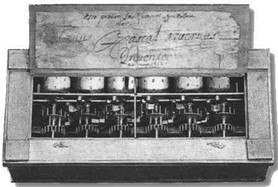
\includegraphics{images_2_cap/1-pascalina.jpg}

}

\caption{Imagen de la Pascalina}

\end{figure}%

A principios del siglo XVI las computadoras se comenzaron a utilizar con
\emph{fines demográficos} para la realización de censos poblacionales.
Con la incorporación de \emph{tarjetas perforadas} a los dispositivos se
inició una nueva generación de computadoras, en tanto estas podían
realizar cálculos más complejos y agregar más funciones a las
habituales. Las funciones que se incorporaron ya no eran solamente suma,
resta, multiplicación y división, sino también raíz cuadrada, conversión
de decimal a binario, funciones logarítmicas y trigonométricas,
incorporación de sumas con numeraciones con mayor cantidad de dígitos,
etc., utilizadas frecuentemente para contabilizar y registrar la
cantidad de habitantes en una región, entre otras cosas.

Las tarjetas perforadas serían utilizadas para almacenar los
\emph{``programas''} de la máquina, quien le daba las instrucciones para
operar. Asimismo, fueron adoptadas por la industria de los telares para
que un hilador pudiera producir telas sin necesidad de un asistente. Fue
Joseph Jacquard quien diseñó un modelo donde la tarjeta estaba colgada
sobre un tambor rotatorio para controlar el hilo en forma automática. De
ahí el nombre de la tela.

\begin{figure}[H]

{\centering 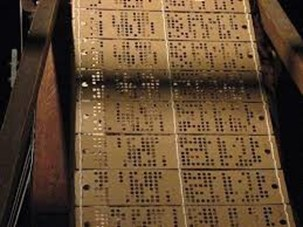
\includegraphics{images_2_cap/2-tarjetas-perforadas.jpg}

}

\caption{Tarjetas Perforadas}

\end{figure}%

En 1820 el británico Charles Babbage propone la \emph{``máquina
diferencial''} a la Real Sociedad Astronómica de Londres. Definida como
``\emph{la máquina que se come su propia cola''} realizaba operaciones
complejas en forma automatizada en base a un sistema de
retroalimentación. Era un dispositivo con memoria, es decir, donde los
números fueran almacenados en registros, denominados almacenes. El
mecanismo fue denominado ``la cadena'' donde una especie de rodillo
podía moverse mediante una fuerza aplicada en sus extremos. ``El
molino'' era la otra parte además del almacén donde se realizarían las
operaciones aritméticas. Si se establece una analogía con la computadora
personal moderna, el molino sería la unidad de procesamiento (CPU)
mientras que el almacén, la memoria RAM.

\begin{figure}[H]

{\centering 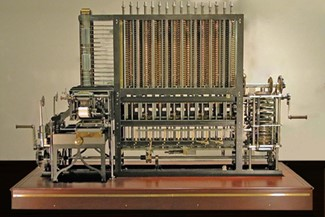
\includegraphics{images_2_cap/3-la-cadena-memoria-ram.jpg}

}

\caption{``La Cadena'' - Máquina Diferencial}

\end{figure}%

Pero fue recién en el Siglo XX en el período de entreguerras, más
específicamente durante la década de 1930 cuando las fuerzas armadas y
agencias de seguridad de países desarrollados comienzan a interesarse
por el uso de computadoras con fines militares. Es aquí donde comienza
una fuerte inversión por parte de los gobiernos de las principales
potencias mundiales en investigación y desarrollo para la creación de
supercomputadoras que tengan objetivos bélicos apoyado en laboratorios
de investigación de empresas contratistas y universidades.

Es así como el complejo militar-industrial va a ser condicionante para
el desarrollo de la computación moderna.

\section{\texorpdfstring{\textbf{El complejo militar industrial y el
desarrollo de la computación
moderna}}{El complejo militar industrial y el desarrollo de la computación moderna}}\label{el-complejo-militar-industrial-y-el-desarrollo-de-la-computaciuxf3n-moderna}

La inversión gubernamental de las grandes potencias para el desarrollo
de supercomputadoras que cumplan funciones militares demuestra la fe
depositada en la tecnología para hacer ganar una guerra a un país o una
nación. Apoyada en el trabajo conjunto con los laboratorios de
investigación de grandes firmas privadas y de las universidades, esta
alianza tuvo su correlato en la realización de grandes innovaciones
tecnológicas que dieron lugar al desarrollo de la computación moderna.
En los Estados Unidos existen tres ejemplos paradigmáticos que son el
Instituto de Tecnología de Massachussets (MIT) y los Laboratorios Bell.

El MIT es una de las instituciones de educación universitaria con sede
en Cambridge, Massachusetts más importante del mundo en materia de
tecnología que ha desarrollado importantes innovaciones a partir del
financiamiento gubernamental y empresarial. Creada en 1861 como
institución privada, en pleno desarrollo industrial de los Estados
Unidos, su objetivo era realizar investigaciones que favorecieran el
cambio tecnológico de la época. Si bien funciona como una universidad
politécnica, se destacada en el campo de la ingeniería. Su desarrollo
histórico creció exponencialmente a partir de su intromisión en el
desarrollo militar durante la Segunda Guerra Mundial. Durante el
conflicto bélico administró el Laboratorio de Radiación, el principal
centro de investigación y desarrollo de radares de los Estados Unidos.
En la posguerra, el instituto colaboró estrechamente para el
departamento de Defensa de los EE. UU. en el desarrollo de la
computación, Internet y programas varios, como en el área de
Inteligencia Artificial, donde en 1957 John McCarthy crea el primer
laboratorio del país desde donde se realizaron varias investigaciones
aplicadas al campo militar.

Ya durante la década del 60, varios de sus miembros trabajaron en forma
asociada para el gobierno de los Estados Unidos para el desarrollo de la
red de computadoras militares ARPANET, donde se desarrolló la teoría de
conmutación para la transmisión de datos mediante paquetes de
información suplantando los circuitos eléctricos. En el área de la
informática interactiva, fue Larry Roberts, ingeniero del instituto,
quien realizó la primera conexión de la historia entre Massachusetts y
California desde la Oficina de Técnicas de Procesamiento de la
Información de ARPA, la Agencia de proyectos Avanzados del Departamento
de

Defensa. Asimismo, el término hacker aparece por primera vez a partir de
la auto denominación de los programadores informáticos MIT a partir de
la admiración que les producían los técnicos de la empresa de telefonía
norteamericana ATT de arreglar ``a golpes de hachazos'' las cajas de los
postes callejeros.

Otro centro de investigación privado son los laboratorios de la empresa
de telefonía Bell Corporation. Fundado en 1925, los ``Bell Lab'' se
crearon por iniciativa del dueño de la patente del teléfono, Alexander
Graham Bell al comprar acciones en la compañía Western Electric,
asociada a AT\&T, donde a partir de entonces ambas compañías acuerdan
financiar la creación de este centro. La mayoría de las innovaciones de
los laboratorios Bell se orientan a las comunicaciones, donde se destaca
la instalación de cables submarinos para las comunicaciones telefónicas
intercontinentales en 1927 y los satélites de telecomunicaciones, cuando
a través del TELSTAR 1 se transmitieron imágenes de televisión y
llamadas telefónicas a través del espacio. El cine también fue parte de
las innovaciones del centro cuando en 1926 se desarrolló el sistema de
grabación y reproducción de sonido con imágenes en movimiento.

Pero la invención más destacada para el desarrollo de supercomputadoras
fue el transistor en 1947, donde se dio inicio a una nueva generación de
computadoras al sustituir los tubos de vacío por los cuales funcionaban
hasta ese momento. Asimismo, bajo financiación gubernamental, el
laboratorio también participo en el diseño de la tecnología de
conmutación para la trasmisión digital de datos en redes de telefonía en
1962. Además de diversas publicaciones científicas y técnicas realizadas
por encargo del Departamento de Defensa de los Estados Unidos en la
actualidad, el centro se encuentra bajo la órbita de la empresa Alcatel
Lucent y es pionera en las investigaciones para incrementar la velocidad
de transmisión de datos en las redes, telefonía celular y
telecomunicaciones en general.

\section{\texorpdfstring{\textbf{La creación de supercomputadoras
militares}}{La creación de supercomputadoras militares}}\label{la-creaciuxf3n-de-supercomputadoras-militares}

En cuanto a los fines militares de las computadoras, en líneas
generales, los mismos estaban orientados a dos objetivos:

\begin{itemize}
\item
  En materia balística: para calcular la trayectoria de los proyectiles
  por parte de la artillería en conflictos bélicos;
\item
  En materia de seguridad de las comunicaciones: para cifrar los
  mensajes del ejército a partir del uso de la criptografía.
\end{itemize}

En materia balística, en 1939 los Laboratorios Bell diseñaron para el
Comité para la Investigación para la Defensa Nacional de los Estados
Unidos una computadora que permitía fijar en forma automática el blanco
de la artillería antiaérea. La \emph{Complex Number Computer} funcionó
de 1940 a 1950 en el laboratorio del Ejército norteamericano. En 1944,
IBM pone en funcionamiento la computadora \emph{Mark I}, financiada por
el Gobierno para solucionar problemas de balística y diseño naval al
final de la Segunda Guerra Mundial.

En materia de seguridad de las comunicaciones hubo una amplia inversión
en la creación de supercomputadoras criptográficas2.

El desarrollo de las maquinas criptografías se inicia en 1919 en
Alemania, cuando la compañía Heimsoeth \& Rinke crea la máquina
\emph{Enigma}, una computadora capaz de cifrar mensajes mediante
técnicas de sustitución criptográficas. Tras el fracaso comercial fue
vendida al Ejército alemán en 1928 y posteriormente utilizada en la
Segunda Guerra Mundial. Es justamente durante dicho conflicto bélico que
se desarrolló la criptografía moderna, basada en estudios científicos
provenientes de diferentes disciplinas como la matemática Discreta, la
Teoría de los Grandes Números y las Ciencias de la Computación.

En 1939 los servicios de inteligencia inglés y francés fueron invitados
por su símil de Polonia a una reunión secreta para mostrarles el
funcionamiento de unas máquinas de desciframiento llamadas ``bombas'',
una de las cuales venían decodificando los mensajes de la Enigma
mediante la simulación del movimiento de los rotores de esta. El motivo
de la reunión fue compartir la información con esos países ante la
inminencia del estallido de la guerra. En 1940, el matemático ingles
Alan Turing elaboraría una versión mejorada de estas máquinas. La bomba
inglesa media 2,40 de alto y 2.40 de diámetro y fue la primera máquina
electromecánica dedicada al criptoanálisis\textbf{.}

\begin{figure}[H]

{\centering 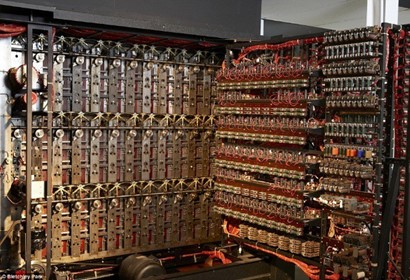
\includegraphics{images_2_cap/4-primeras-supercomputadoras.jpg}

}

\caption{Supercomputadora Criptográfica}

\end{figure}%

En ese entonces se comenzaron a utilizar las maquinas que se encargaban
de cifrar los mensajes basadas en la técnica de discos rotativos, como
la TYPEX británica o la Converter M-209 estadounidense. En 1943 en
Inglaterra se pone en funcionamiento la computadora
\emph{Colossus}\textbf{,} una máquina descifradora automática. Una vez
finalizada la contienda mundial, el primer ministro británico Winston
Churchill ordenó la destrucción de las 10 Colossus operativas y decretó
el secreto de funcionamiento por 30 años.

\section{\texorpdfstring{\textbf{Historia de Internet y la World Wide
Web}}{Historia de Internet y la World Wide Web}}\label{historia-de-internet-y-la-world-wide-web}

La historia de Internet comienza durante la denominada Guerra Fría, un
enfrenamiento bélico no declarado que se inicia a partir de 1945 entre
las dos potencias victoriosas de la Segunda Guerra Mundial: los Estados
Unidos y La Unión Soviética, basado en un enfrentamiento político entre
el sistema capitalista y el comunismo soviético. Pero fue recién en 1957
cuando la URSS lanza al espacio el satélite Sputnik cuando comienza una
batalla entre ambas potencias en el plano tecnológico. Un año después de
este acontecimiento, el presidente norteamericano Dwight Eisenhower
ordena la creación de una agencia de investigación y desarrollo (I+D)
para la realización de estudios sobre material bélico y comunicaciones.
Es así como en 1958 se crea la Agencia de Investigación de Proyectos
Avanzados (ARPA) en el seno del Departamento de Defensa de los Estados
Unidos.

Joseph Licklider, psicólogo e investigador asociado del MIT es nombrado
Director del Programa de Investigación Informática de ARPA con el objeto
de mejorar las comunicaciones del ejército a través de computadoras. En
1962 presenta una serie de memorándums para crear una red de
computadoras bajo el nombre de ``Red Galáctica''. Por aquel entonces
imaginó un conjunto de computadoras conectadas entre sí globalmente por
donde se podía acceder a datos e información y al uso compartido de
programas desde todo el mundo. Dos años más tarde, en 1964, Leonard
Kleinrock -ingeniero eléctrico e investigador también del MIT- publica
un libro sobre la teoría de la conmutación de paquetes donde afirmaba
que era factible que las computadoras se comuniquen entre sí a través de
paquetes de datos y no de circuitos eléctricos.

Al año siguiente, en 1965 el ingeniero Larry Roberts, del mismo
instituto, realizó una prueba piloto desde la Oficina de Técnicas de
Procesamiento de la Información (IPTO) conectando dos computadoras entre
Massachusetts y California e intercambiando datos. Es allí donde se
estableció la primera comunicación entre computadoras de la historia. La
interconexión se realizó mediante una línea telefónica conmutada. Fue la
primera red de computadoras de tiempo compartido donde podían ejecutar
programas al mismo tiempo en forma remota (a distancia) e intercambiar
datos entre sí.

Tras estos hechos, el Departamento de Defensa aprueba la realización de
una red de computadoras con un objetivo militar: la creación de un medio
de comunicación flexible y descentralizado que sirva como medio de
comunicación alternativo a los sistemas de telecomunicaciones
tradicionales (teléfono, telégrafo). Este objetivo partía de la
hipótesis de un posible conflicto bélico dentro del territorio
norteamericano que colapsara las comunicaciones internas,
fundamentalmente frente a un posible ataque nuclear soviético.

Pero fue recién en 1969 que se establecieron conexiones fijas entre la
Universidad de California (UCLA) y el Instituto de Investigación de
Stanford (SRI) de la Universidad de Utah y la Universidad de Santa
Bárbara de California Estableciéndose como nodos principales, se da
inicio a ARPANET, la red de computadoras militares de ARPA.

\begin{figure}[H]

{\centering 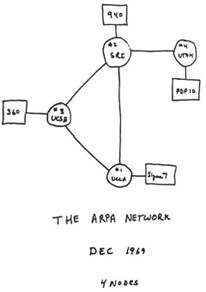
\includegraphics{images_2_cap/5-nodos-ARPA.jpg}

}

\caption{Bosquejo Original - NODOS ARPA}

\end{figure}%

Ya durante la década siguiente, en 1972 se inicia el Programa
\emph{Internetting con el} objetivo de establecer una red de
\emph{``arquitectura abierta}'' que tenga como centro de interconexión a
ARPANET. Una red de redes donde cada una mantenga su propia estructura y
configuración. Reglas básicas del Programa eran:

\begin{enumerate}
\def\labelenumi{\arabic{enumi}.}
\item
  Cada red debía mantenerse por sí misma y no debía haber cambio alguno
  para que pudiera conectarse a Internet.
\item
  La comunicación debía hacerse en base al mejor esfuerzo (``best
  effort'') si un paquete de datos no llegaba a destino debía
  retransmitirse desde el origen.
\item
  Se usarían cajas negras para interconectar las redes (puertas de
  enlace y enrutadores) sin que guarden información sobre los paquetes
  de datos.
\item
  No debía haber control global a nivel operativo
\end{enumerate}

Tras el desarrollo de diferentes innovaciones tecnológicas en el área de
la informática interactiva y el surgimiento de nuevas redes
organizacionales, el Departamento de Defensa de los EE. UU. -preocupado
por la seguridad de las comunicaciones- crea en 1983 MILNET, una red
subsidiaria de ARPANET para investigaciones militares. Librada de fines
militares, la red pasó a llamarse ARPANET-INTERNET con fines de
investigación académica.

\begin{figure}[H]

{\centering 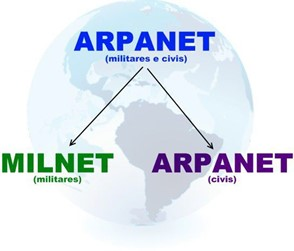
\includegraphics{images_2_cap/6-ARPANET-MILNET.jpg}

}

\caption{Migración de ARPANET a MILNET}

\end{figure}%

En términos políticos, en 1985 asume Mikail Gorvachov como Secretario
General del Partido Comunista en la Unión Soviética. Un año más tarde se
produce la explosión en la planta nuclear de Chernobyl, hecho que
aceleró un proceso de reforma de la economía soviética conocida como
``Perestroika (reestructuración, en ruso). Esto marca el inicio de una
distensión política entre los Estados Unidos y la Unión Soviética a
partir de un acercamiento entre los presidentes de ambos países George
Bush y Gorbachov. Estados Unidos se identifica victorioso de la
contienda política y la competitividad tecnológica y no percibe a la
URSS como una amenaza en términos militares.

En este contexto la Fundación Nacional de la Ciencia (NSF, sus siglas en
inglés) de los Estados Unidos solicita autorización al Congreso de ese
país para construir una red de computadoras científica a nivel nacional
para toda la comunidad académica y de investigación del país. Es así
como al año siguiente se crea NSFNET, la Red para la Ciencia Nacional.

En 1988 se crea el \emph{Commercial Internet Exchange}, un consorcio de
proveedores de redes comerciales y regionales para la explotación
privada de la red. Su objetivo era brindar servicio de acceso comercial
a la red más allá de la NSFNET. Bajo el nombre \emph{``La
comercialización y privatización de Internet''} se inician conferencias
en Harvard. El Senador Al Gore elaboró un proyecto para la creación de
la Infraestructura Nacional de la Información (NNI) para el desarrollo
de las \emph{autopistas de la información.}

Por otro lado, a mediados de los 80s, Tim Berners Lee, un físico
británico ingresa al Área de Conexiones de Red del Centro para la
Investigación Nuclear Europeo (CERN) con el fin de diseñar un sistema
informático que permitiese solucionar la dispersión de documentación
almacenada en diferentes computadoras de la organización. Su proyecto
constaba del desarrollo de un programa llamado Enquire Within Upon
Everything (``Pregunte acerca de todo'') y permitiría el intercambio
automatizado de información y la consulta por Internet durante las 24
horas. Pero el CERN le asignó una importancia secundaria y Berners Lee
partió de la organización.

El programa estaba basado en la idea del hipertexto, desarrollada por el
ingeniero del MIT Vannevar Bush en 1945 en un artículo titulado ``As We
May Thing'' (Como podemos pensar) publicado en The Atlantic Monthy. Para
Bush - quien formó parte del Proyecto Manhattan que diseñó la bomba
atómica para los Estados Unidos- ``La mente humana funciona por
``asociación'' de ideas a través de una red de caminos de células del
cerebro''. Tradicionalmente la información se clasifica alfabética y
numéricamente y se organiza jerárquicamente siguiendo la pauta de grupos
o clases. Para este ingeniero se debía trabajar a partir de la
Indexación, donde cualquier elemento puede ser enlazado automáticamente
a otro del acuerdo al interés de conocimiento.

Bush imagino la creación de un dispositivo llamado \emph{Memex} que
tenga la \textbf{c}apacidad de almacenar información textual y grafica
donde cualquier pieza se pueda vincular entre si arbitrariamente, se
puedan añadir notas marginales aprovechándose de fotografías y el acceso
a la información mediante ``enlaces'' por el cual luego podía ser
recuperada desde el origen. Memex iba a estar compuesto por un
escritorio, pantallas translucidas en el que el material es proyectado,
teclados, botones y palancas para establecer una mejor comunicación.

\begin{figure}[H]

{\centering 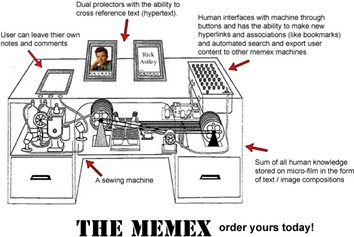
\includegraphics{images_2_cap/7-proyecto-MEMEX.jpg}

}

\caption{Proyecto MEMEX}

\end{figure}%

Si bien la idea de de un hipertexto fue concebida por Bush en 1945, el
término fue acuñado por el filósofo y sociólogo estadounidense Theodore
Nedson en 1965 en un paper escrito para la Revista \emph{Literary
Machines.} El hipertexto es una Forma de escritura no lineal o
secuencial, un tipo de texto que se ramifica y permite la elección al
lecto y funciona a través de una pantalla interactiva. En el artículo
describe una máquina concebida teóricamente en 1960 por Nelson bajo el
nombre Proyecto Xanadú, que constaba de una base de datos universal de
conocimiento fundado en un archivo de documentos (``docuverso'') donde
los archivos se encadenan entre sí a modo de enlace directo entre citas
y notas de texto.

En 1989 Tim Berners Lee regresa al CERN presenta el proyecto Information
Management: A Proposal (``Una propuesta para la gestión de
información'') donde propone la creación de una infraestructura mundial
de información con el objetivo de solucionar las deficiencias en la
entrega de información entre los diferentes centros de investigación del
CERN. Basado en la tecnología del hipertexto, el sistema permitiría el
intercambio automatizado de información y la consulta de documentación
por Internet durante las 24 horas. El proyecto fue aprobado por las
autoridades del Centro, recibió financiamiento necesario para comenzarlo
un año más tarde y el nombre del programa fue reformulado al de World
Wide Web. El mismo constaba de un programa navegador, un Lenguaje
informático para su funcionamiento (HTML), un Protocolo de
comunicaciones (HTTP) y un sistema de Sistema de direcciones (URLs).

\textbf{Recuerde:} En cada imagen existe una fuente de consulta, la
misma que de alguna forma podría ampliar su conocimiento.

No olvide que sus aportes son muy valiosos, para el desarrollo de este
texo.

\bookmarksetup{startatroot}

\chapter{Introduction}\label{introduction}

This is a book created from markdown and executable code.

See Knuth (1984) for additional discussion of literate programming.

\bookmarksetup{startatroot}

\chapter{Summary}\label{summary}

In summary, this book has no content whatsoever.

\bookmarksetup{startatroot}

\chapter*{References}\label{references}
\addcontentsline{toc}{chapter}{References}

\markboth{References}{References}

\phantomsection\label{refs}
\begin{CSLReferences}{1}{0}
\bibitem[\citeproctext]{ref-knuth84}
Knuth, Donald E. 1984. {``Literate Programming.''} \emph{Comput. J.} 27
(2): 97--111. \url{https://doi.org/10.1093/comjnl/27.2.97}.

\end{CSLReferences}




\end{document}
